\section{I/O Systems}\label{sec:IO_Systems}
Because I/O devices vary so widely in their function and speed, varied methods are needed to control them.
These methods form the I/O subsystem of the kernel, which separates the rest of the kernel from the complexities of managing I/O devices.

To encapsulate the details and oddities of different devices, the kernel of an operating system is structured to use \nameref{def:Device_Driver} modules.

\begin{definition}[Device Driver]\label{def:Device_Driver}
  \emph{Device Driver}s present a uniform device-access interface to the I/O subsystem.
  Every device requires a device driver (though certain devices can reuse another device's driver).
  The device driver hides the device-specific implementation details from the \nameref{def:Operating_System} and I/O subsystem, and only showing a standard, uniform interface.
  The type of interface exported depends on the nature of the device itself.

  This is analogous to \nameref{def:System_Call}s providing a standard interface between the application and the \nameref{def:Operating_System}.
\end{definition}

Despite the incredible variety of I/O devices, though, we need only a few concepts to understand how the devices are attached and how the software can control the hardware.

\subsection{I/O Hardware}\label{subsec:IO_Hardware}
The device communicates with the machine via a connection point, a port.
If devices share a common set of wires, the connection is called a \nameref{def:Hardware_Bus}.
Buses are used widely in computer architecture and vary in their signaling methods, speed, throughput, and connection methods.

\begin{definition}[Bus]\label{def:Hardware_Bus}
  A \emph{bus} is a set of wires and a rigidly defined protocol that specifies a set of messages that can be sent on the wires.
\end{definition}

When device A plugs into device B, and device B plugs into device C, and device C plugs into a port on the computer, this arrangement is called a daisy chain.
A daisy chain usually operates as a \nameref{def:Hardware_Bus}.

All of these may be controlled by a \nameref{def:Controller}.

\begin{definition}[Controller]\label{def:Controller}
  A \emph{controller} is a collection of electronics that can operate a port, a \nameref{def:Hardware_Bus}, or a device.
\end{definition}

Because some protocols are complex, their \nameref{def:Hardware_Bus} \nameref{def:Controller} is often implemented as a separate circuit board (or a host adapter) that plugs into the computer.
It typically contains a processor, microcode, and some private memory to enable it to process the protocol messages.
Some devices have their own built-in controllers.
They can receive commands in 2 ways (some support both, some do not):
\begin{enumerate}[noitemsep]
\item The \nameref{def:Controller} has one or more registers for data and control signals.
  The processor communicates with the controller by reading and writing bit patterns in these registers.
  This communication can occur through the use of special I/O instructions that specify the transfer of a byte or word to an I/O port address.
  The I/O instruction triggers bus lines to select the proper device and to move bits into or out of a device register.
\item The device \nameref{def:Controller} can support \nameref{subsubsec:Memory_Mapped_IO}.
  In this case, the device-control registers are mapped into the address space of the processor.
  The CPU executes I/O requests using the standard data-transfer instructions to read and write the device-control registers at their mapped locations in physical memory.
\end{enumerate}

For example, a graphics controller supports both of these methods of control.
\begin{itemize}[noitemsep]
\item The graphics controller has I/O ports for basic control operations.
\item The controller has a large memory-mapped region to hold screen contents.
  The process sends output to the screen by writing data into the memory-mapped region.
  The controller generates the screen image based on the contents of this memory.
\end{itemize}

The ease of writing to a \nameref{subsubsec:Memory_Mapped_IO} \nameref{def:Controller} is offset by the disadvantage of being vulnerable to accidental modification by an incorrect pointer to an unintended region of memory.
Memory protection helps reduce this risk.

\subsubsection{I/O Ports}\label{subsubsec:IO_Ports}
An I/O port typically consists of four registers, called the status, control, data-in, and data-out registers.
\begin{enumerate}[noitemsep]
\item The \textbf{\texttt{data-in} register} is read by the host to get input.
\item The \textbf{\texttt{data-out} register} is written by the host to send output.
\item The \textbf{\texttt{status} register} contains bits that can be \textbf{read by the host}.
  These bits indicate states, such as:
  \begin{itemize}[noitemsep]
  \item Whether the current command has completed.
  \item Whether a byte is available to be read from the data-in register.
  \item Whether a device error has occurred.
  \end{itemize}

\item The \textbf{\texttt{control} register} can be \textbf{written by the host} to start a command or to change the mode of a device.
  For instance:
  \begin{itemize}[noitemsep]
  \item One bit in a register of a serial port chooses between full-duplex and half-duplex communication.
  \item Another bit enables parity checking.
  \item A third bit sets the word length to different bit lengths.
  \item Other bits select one of the speeds supported by the serial port.
  \end{itemize}
\end{enumerate}

\subsubsection{Polling}\label{subsubsec:Polling}
The controller indicates its state through the \texttt{busy} bit in the \texttt{status} register.
The controller sets the \texttt{busy} bit when it is busy working and clears it when the controller is ready to accept the next command.
The host signals its wishes by setting the \texttt{command-ready} bit in the \texttt{command} register when a command is available for the controller to execute.

The repeating loop of polling is described in the following steps:
\begin{enumerate}[noitemsep]
\item The host repeatedly reads the \texttt{busy} bit until that bit becomes clear.
\item The host sets the \texttt{write} bit in the \texttt{command} register and writes a byte into the \texttt{data-out} register.
\item The host sets the \texttt{command-ready} bit.
\item When the controller notices that the \texttt{command-ready} bit is set, it sets the busy bit.
\item The controller reads the \texttt{command} register and sees the \texttt{write} command.
  It reads the \texttt{data-out} register to get the byte and does the I/O to the device.
\item The controller clears the \texttt{command-ready} bit, clears the error bit in the status register to indicate that the device I/O succeeded, and clears the \texttt{busy} bit to indicate that it is finished.
\end{enumerate}

The host is \textbf{busy-waiting} or \textbf{polling} in the first step: it is in a loop, reading the status register over and over until the busy bit becomes clear.
If the controller and device are fast, this is reasonable.
But if the wait is long enough, the host should switch to another task.

For some devices, the host \textbf{must} service the device quickly, or data will be lost.
For instance, when data are streaming in on a serial port, the small buffer on the controller will overflow and data will be lost if the host waits too long before returning to read the bytes.

The basic polling operation is instruction-efficient.
In many computer architectures, just three CPU-instruction cycles are sufficient to poll a device:
\begin{enumerate}[noitemsep]
\item Read a device register.
\item Logical \texttt{AND} to extract a status bit.
\item Branch if not zero.
\end{enumerate}

But polling becomes inefficient when it is attempted repeatedly yet rarely finds a device ready for service, while other useful CPU processing remains undone.
In those cases, it is more efficient to have the hardware controller notify the CPU when the device becomes ready again, rather than require the CPU to poll for I/O completion.
The hardware mechanism that enables a device to notify the CPU is called an \nameref{def:Interrupt}.

\subsubsection{Interrupts}\label{subsubsec:Interrupts}
The CPU hardware has a wire called the \nameref{def:Interrupt_Request_Line} that the CPU senses after executing every instruction.

\begin{definition}[Interrupt-Request Line]\label{def:Interrupt_Request_Line}
  The \emph{interrupt-request line} is a dedicated hardware line or \nameref{def:Hardware_Bus} for sending information about exceptional circumstances to the CPU.\@
  The CPU checks this line after \textbf{every} instruction.

  If the line does not contain any information, the CPU continues normal execution.
  If it does contain some information, then the CPU performs a \nameref{def:Context_Switch}.
  However, instead of switching to another \nameref{def:Process}, the CPU jumps to the \nameref{def:Interrupt_Handler}.
\end{definition}

When the CPU detects that a controller has asserted a signal on the interrupt-request line, the CPU performs a state save and jumps to the \nameref{def:Interrupt_Handler} routine at a fixed address in memory.

\begin{definition}[Interrupt Handler]\label{def:Interrupt_Handler}
  The \emph{interrupt handler}:
  \begin{enumerate}[noitemsep]
  \item Determines the cause of the interrupt.
  \item Performs the necessary processing.
  \item Performs a state restore.
  \item Executes a return from interrupt instruction to return the CPU to the execution state prior to the interrupt.
  \end{enumerate}
\end{definition}

The basic loop of an \nameref{def:Interrupt}-driven \nameref{def:Operating_System} is:
\begin{enumerate}[noitemsep]
\item The device controller \textbf{raises} an interrupt by asserting a signal on the \nameref{def:Interrupt_Request_Line}.
\item The CPU \textbf{catches} the interrupt and \textbf{dispatches} it to the \nameref{def:Interrupt_Handler}.
\item The handler \textbf{clears} the interrupt by servicing the device.
\item The CPU returns to normal execution.
\end{enumerate}


%%% Local Variables:
%%% mode: latex
%%% TeX-master: "../../EDAF35-Operating_Systems-Reference_Sheet"
%%% End:


\subsection{Application I/O Interface}\label{subsec:Application_IO_Interface}
The \nameref{def:Operating_System} wants to treat all I/O devices in a standard, uniform way.
Like other complex software-engineering problems, the approach here involves abstraction, encapsulation, and software layering.
Specifically, we can abstract away the detailed differences in I/O devices by identifying a few general kinds, where each is accessed through a standardized set of functions, its \emph{interface}.
The implementation differences are encapsulated in \nameref{def:Kernel_Module}s called \nameref{def:Device_Driver}s that internally are custom-tailored to specific devices but that export one of the standard interfaces.
The software layering used is shown in \Cref{fig:Kernel_IO_Subsystem_Structure}.

\begin{figure}[h!tbp]
  \centering
  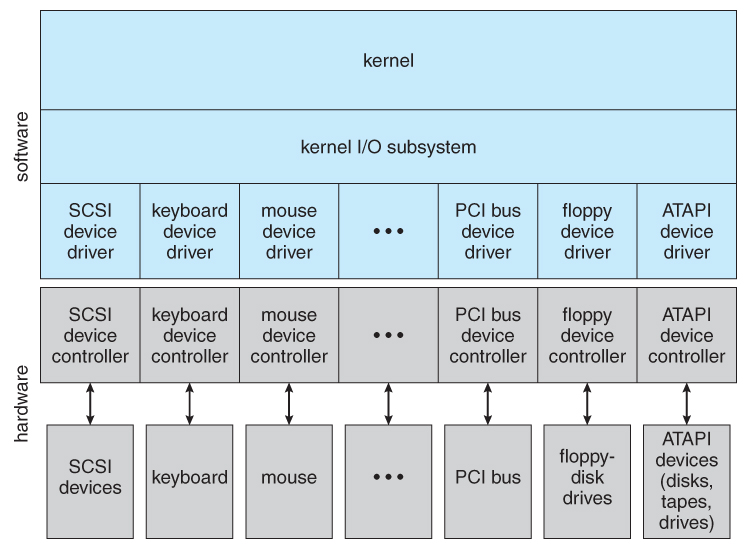
\includegraphics[scale=1.00]{./Drawings/EDAF35-Operating_Systems/Kernel_IO_Subsystem_Structure.jpg}
  \caption{Kernel I/O Subsystem Structure}
  \label{fig:Kernel_IO_Subsystem_Structure}
\end{figure}

This layering methodology is used to hide differences among devices and their controllers from the \nameref{def:Kernel}'s I/O subsystem.
This is analogous to the I/O system calls encapsulating the behavior of devices in a few generic classes that hide hardware differences from applications.

Making the I/O subsystem independent of the hardware simplifies the job of the operating-system developer.
It also benefits the hardware manufacturers.
They either:
\begin{itemize}[noitemsep]
\item Design new devices to be compatible with an existing host controller interface.
\item Write device drivers to interface the new hardware to popular operating systems.
\end{itemize}

Thus, we (users) can attach new peripherals to a computer without waiting for the operating system to develop explicit kernel-level support code.
Unfortunately for hardware manufacturers, each operating system has its own standards for the device-driver interface.

Devices can vary in many dimensions, as seen in \Cref{tab:Characteristics_IO_Devices}.
\begin{table}[h!tbp]
  \centering
  \begin{tabular}{cll}
    \toprule
    \textbf{Aspect} & \textbf{Variation} & \textbf{Example} \\
    \midrule
    \multirow{2}{*}{Data-Transfer Mode} & Character & Terminal \\
                    & Block & Disk \\
    \multirow{2}{*}{Access Method} & Sequential & Modem/Network \\
                    & Random & Magnetic Disk \\
    \multirow{2}{*}{Transfer Schedule} & Synchronous & Magnetic Tape \\
                    & Asynchronous & Keyboard \\
    \multirow{2}{*}{Sharing} & Dedicated & Magnetic Tape \\
                    & Sharable & Keyboard \\
    \multirow{4}{*}{Device Speed} & Latency & \\
                    & Seek Time & \\
                    & Transfer Rate & \\
                    & Delay between Operations & \\
    \multirow{3}{*}{I/O Direction} & & \\
                    & Read-only & CD-ROM (After first write) \\
                    & Write-only & Graphics Controller \\
                    & Read-write & Disk \\
    \bottomrule
  \end{tabular}
  \caption{Characteristics of I/O Devices}
  \label{tab:Characteristics_IO_Devices}
\end{table}

%%% Local Variables:
%%% mode: latex
%%% TeX-master: "../../EDAF35-Operating_Systems-Reference_Sheet"
%%% End:



%%% Local Variables:
%%% mode: latex
%%% TeX-master: "../EDAF35-Operating_Systems-Reference_Sheet"
%%% End:
